\documentclass{article}
\usepackage{import}
\usepackage[ruled]{algorithm2e}
\usepackage[shortlabels]{enumitem}
\usepackage{hyperref}
\usepackage{minted}
\usepackage{subcaption}

\hypersetup{
    colorlinks=true,
    linkcolor=blue,
    filecolor=magenta,      
    urlcolor=cyan,
    pdftitle={Overleaf Example},
    pdfpagemode=FullScreen,
    }
\subimport*{}{macro}

\setlength\parindent{0px}

\begin{document}
\setcounter{problem}{0}
\title{Homework \#2}
\author{
    \normalsize{AA 597: Networked Dynamics Systems}\\
    \normalsize{Prof. Mehran Mesbahi}\\
    \normalsize{Due: Jan 20, 2024 11:59pm}\\
    \normalsize{Soowhan Yi}
}
\date{{}}
\maketitle

\begin{problem}
    Write a code that implements breadth first search to determine if two nodes in a graph are connected by a walk. The input to the code is a list adjacency of the graph (so a dictionary that has the list of nodes and and their respective neighbors), and the desired pair of nodes. The output of the code should come back with the answer that lists either the sequence of adjacent nodes that allows a walk from one node to the next or a message that these two nodes are not connected.  Show how the algorithm works on a few generated graphs on five nodes.
\begin{minted}{python}
"""Breath First Search
    Args:
        G (nx.Digraph): an directed graph with n nodes. 
        desired_nodes ([nx.Digraph.node, nx.Digrapoh.node]):  
        [0]: source node, [1]: destination node
    Returns:
        Tuple(np.list, np.list):
        [0]: Either the sequence of walk to destination or the trial path with statement for failure. 
        [1]: list of nodes for BFS
    """
import util
def bfs_search(G, desired_nodes):
    source = desired_nodes[0]
    destination = desired_nodes[1]
    stateQueue = util.Queue()
    pathQueue= util.Queue()
    visitedSet = []
    visitedSet = set(visitedSet)
    pathList = []
    while source != destination:
        if source not in visitedSet:       
            visitedSet.add(source)
            successors = G[source]
            for successor in successors:
                stateQueue.push(successor)
                pathQueue.push(pathList + [[source, successor]])
        if stateQueue.isEmpty(): 
            print("state queue empty two nodes are not connected.")
            break
        source = stateQueue.pop()
        pathList = pathQueue.pop()
    nodeList = util.np.zeros(len(pathList)+1)
    nodeList[0] = pathList[0][0]
    for i in range(0, len(pathList)):
        nodeList[i+1] = pathList[i][1]
    return pathList, nodeList    
\end{minted}
\begin{figure*}[!h]
    \centering
    \begin{subfigure}{0.2\textwidth}
        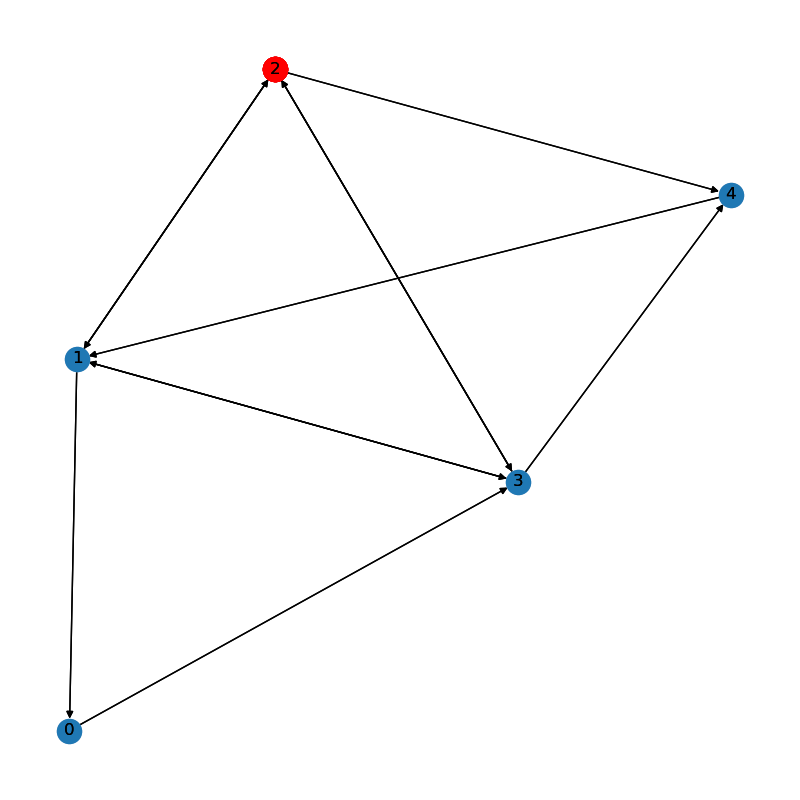
\includegraphics[width=\textwidth]{./img/P1_1/frame0.png}
        \caption{Source = 2}
    \end{subfigure}
    \begin{subfigure}{0.2\textwidth}
        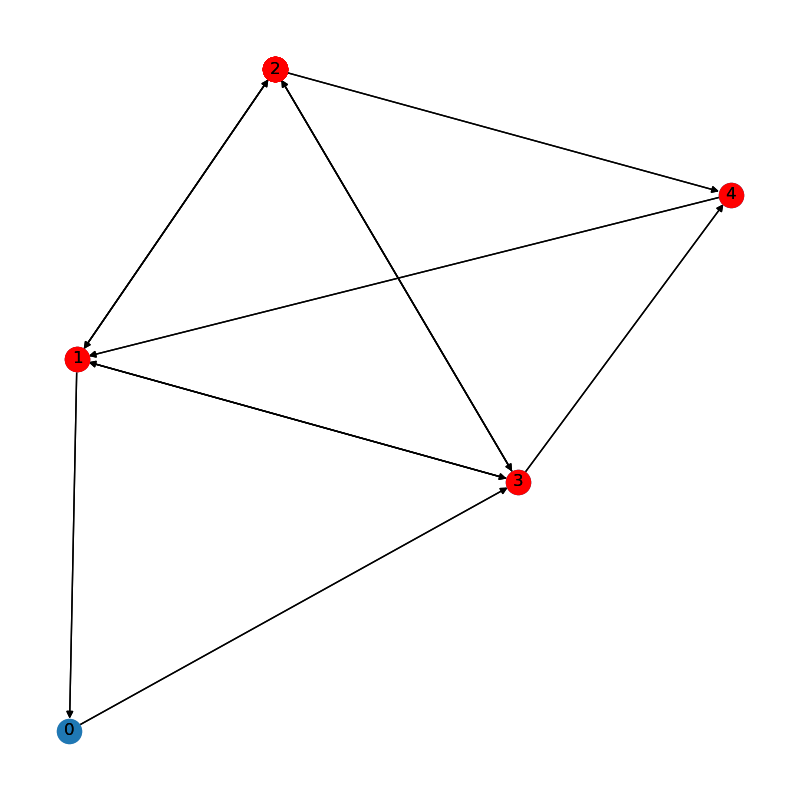
\includegraphics[width=\textwidth]{./img/P1_1/frame1.png}
        \caption{[2,3]}
    \end{subfigure}
    \begin{subfigure}{0.2\textwidth}
        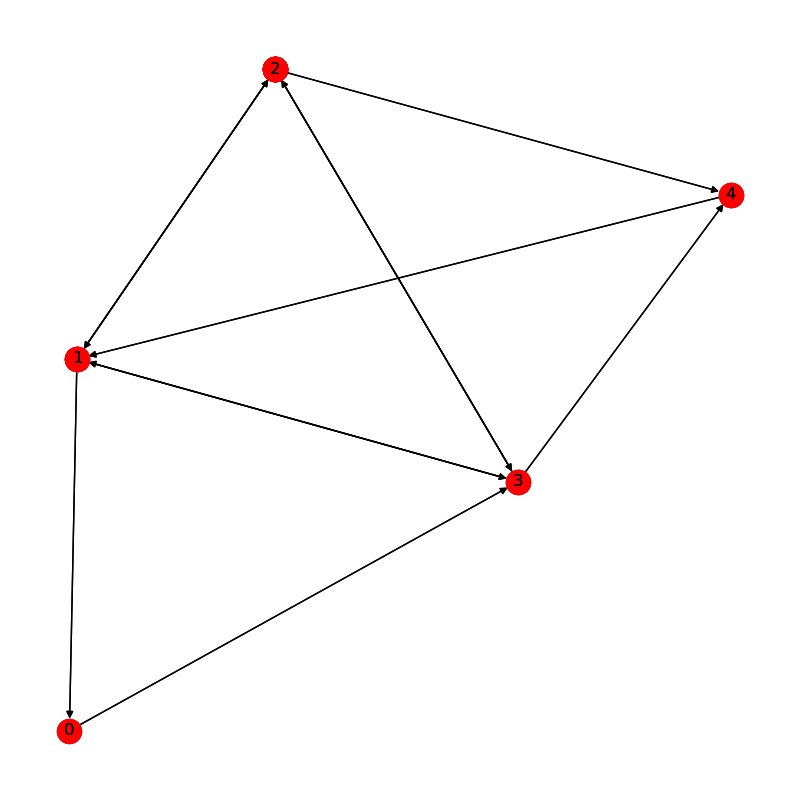
\includegraphics[width=\textwidth]{./img/P1_1/frame2.png}
        \caption{[3,4]}
    \end{subfigure}
\end{figure*}
\begin{figure*}[!h]
    \centering
    \begin{subfigure}{0.2\textwidth}
        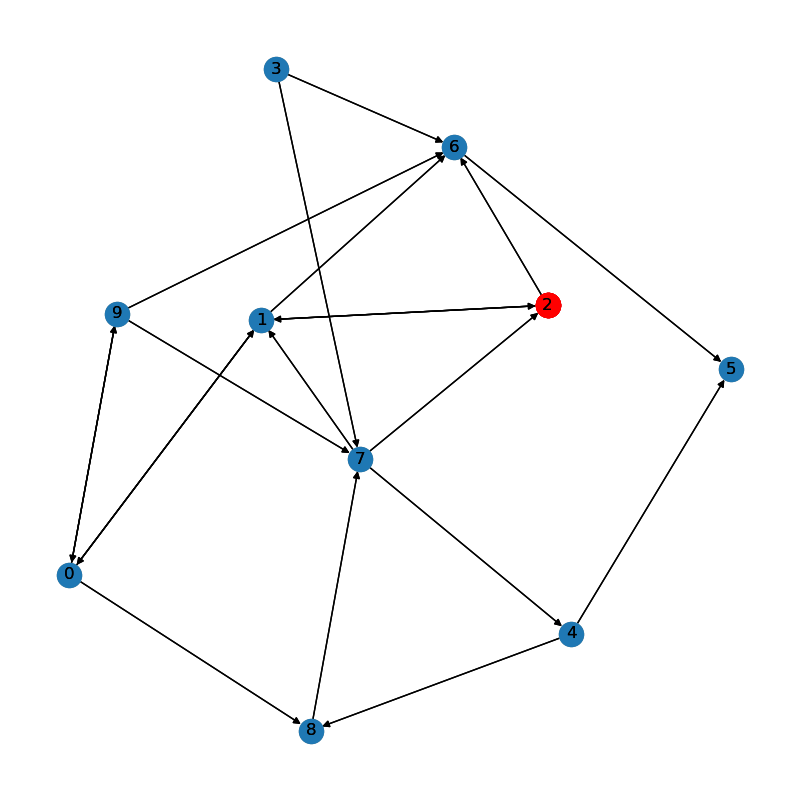
\includegraphics[width=\textwidth]{./img/P1_2/frame0.png}
        \caption{Source =2}
    \end{subfigure}
    \begin{subfigure}{0.2\textwidth}
        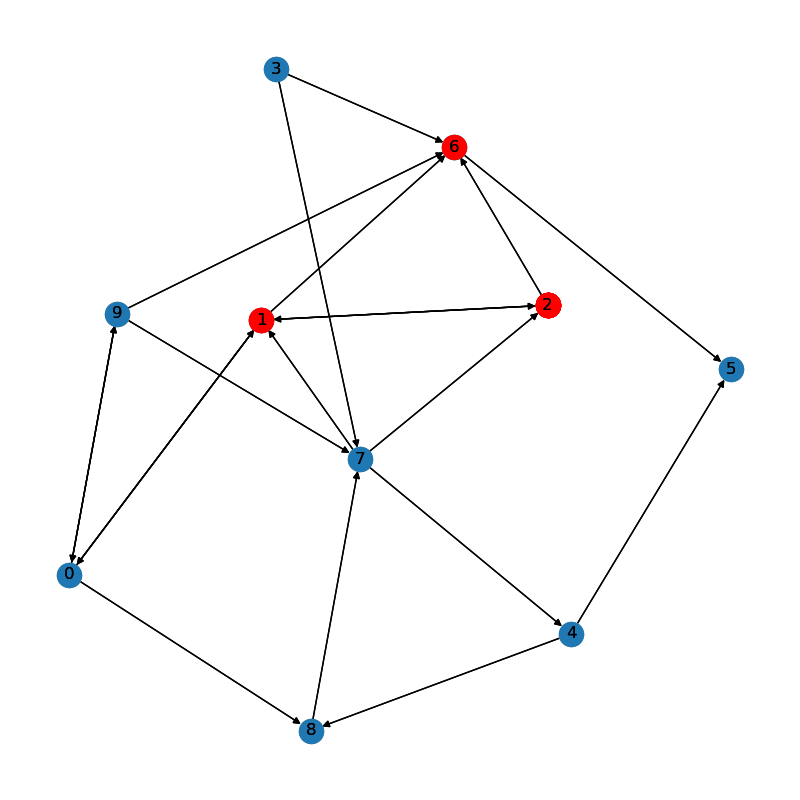
\includegraphics[width=\textwidth]{./img/P1_2/frame1.png}
        \caption{frame 1}
    \end{subfigure}
    \begin{subfigure}{0.2\textwidth}
        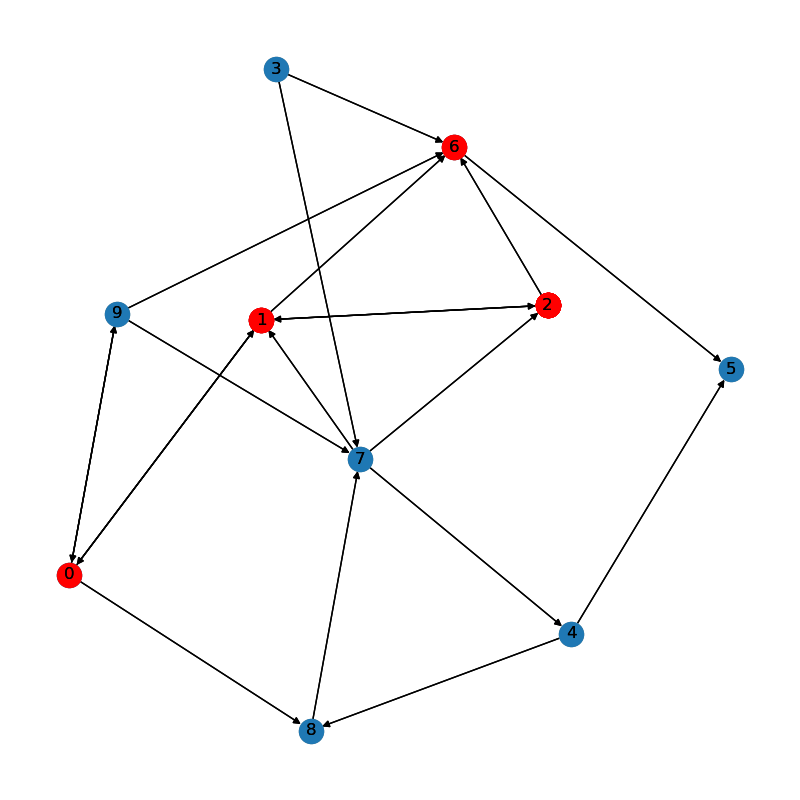
\includegraphics[width=\textwidth]{./img/P1_2/frame2.png}
        \caption{frame 2}
    \end{subfigure}

\end{figure*}

\begin{figure*}[!h]
    \centering
    \begin{subfigure}{0.2\textwidth}
        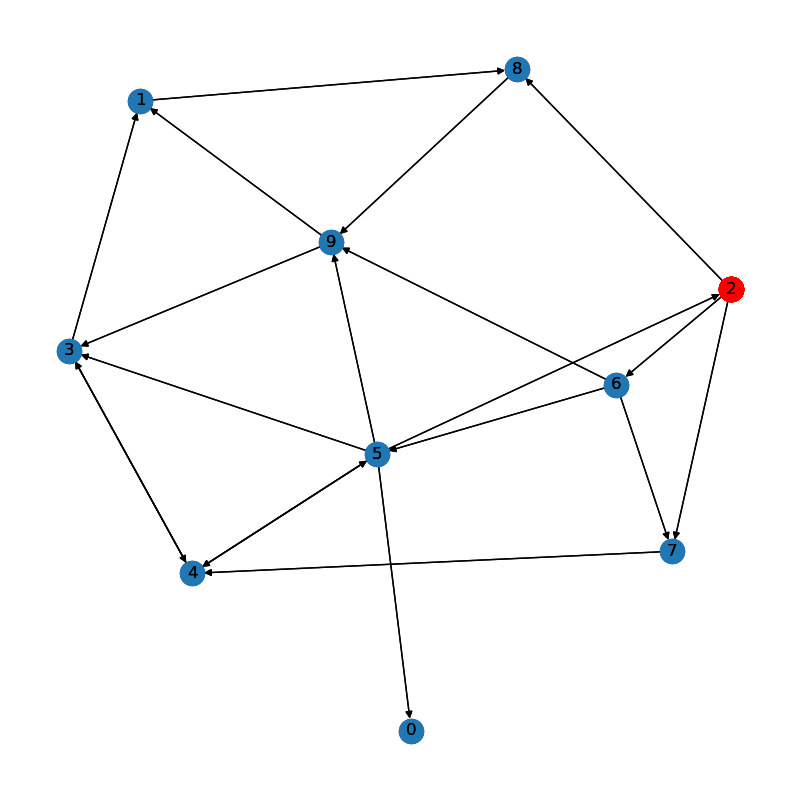
\includegraphics[width=\textwidth]{./img/P1_3/frame0.png}
        \caption{Source =2}
    \end{subfigure}
    \begin{subfigure}{0.2\textwidth}
        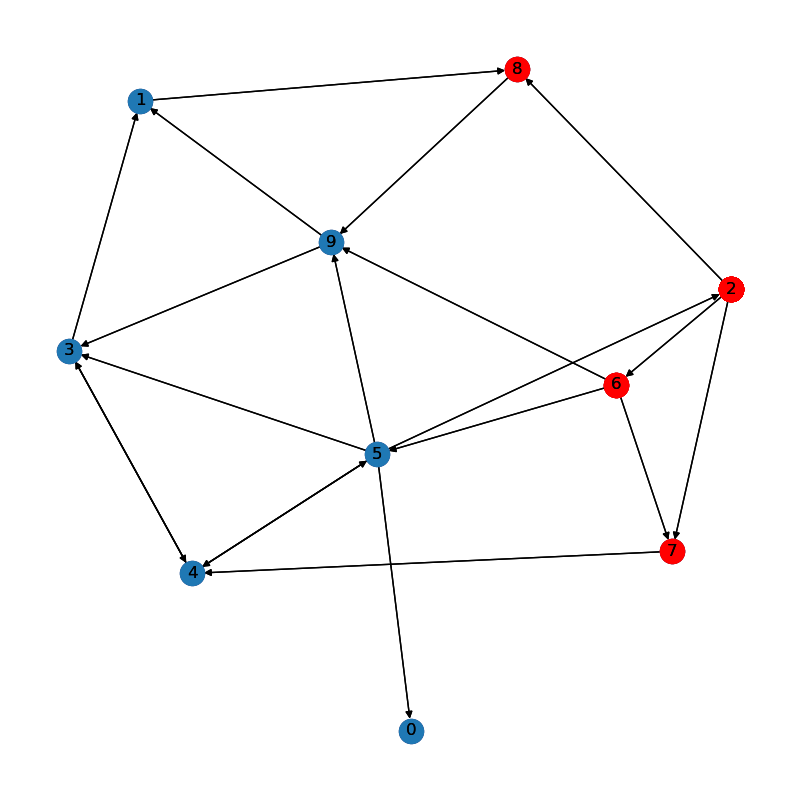
\includegraphics[width=\textwidth]{./img/P1_3/frame1.png}
        \caption{frame 1}
    \end{subfigure}
    \begin{subfigure}{0.2\textwidth}
        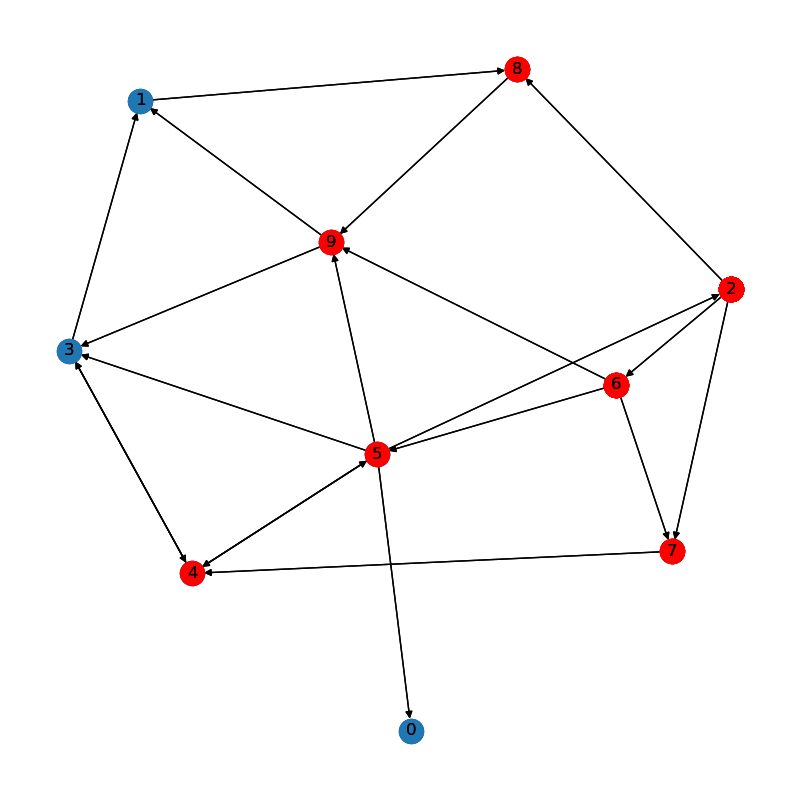
\includegraphics[width=\textwidth]{./img/P1_3/frame2.png}
        \caption{frame 2}
    \end{subfigure}
    \begin{subfigure}{0.2\textwidth}
        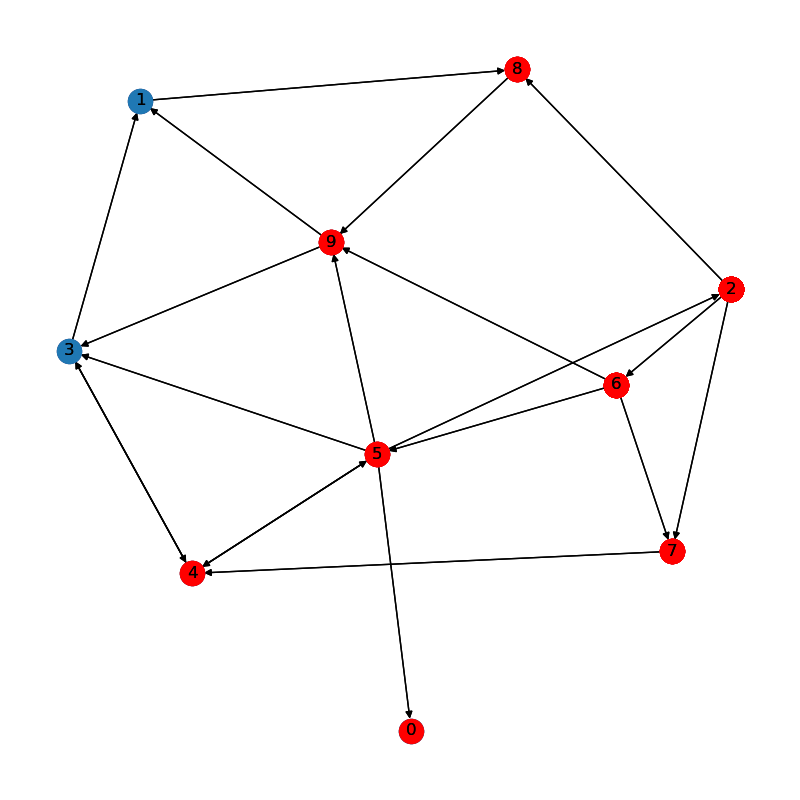
\includegraphics[width=\textwidth]{./img/P1_3/frame3.png}
        \caption{frame 3}
    \end{subfigure}

\end{figure*}
Above figures show how the breath first search works. Those graphs are randomly generated and their edges have directions. Utility file, which includes codes for randomly generated graphs and class for Queue, is also included at the end of the document. Starting from node 2, the search agent looks for the neighbors and put those neighbors into a queue. This queue(first in first out) then pops the next node to search and puts its neighbors to the queue again. This way we can traverse through the graph by searching for the closest neighbor to get to the destination. Here are the links to the video of above simulation.

\url{https://github.com/SoowhanYi94/ME597/tree/ebb5167094092be938096bbc1a82e4b2dce9d7b3/HW1}

\end{problem}

\begin{problem}
    Show the trace $A(G)^3$ (the cube of the adjacency matrix) is six times the number of triangles (cycles with length 3) in the graph G.\\
    Let $A(G) = \begin{bmatrix*}
        a_{11} & a_{12} & \cdots & a_{1n} \\
        a_{11} & a_{22} & \cdots & a_{2n} \\
        \vdots & &&\\
        a_{n1} & a_{n2} & \cdots & a_{nn}
    \end{bmatrix*}$ and $A(G)_{ij} = a_{ij}$.
    \begin{align*}
         A(G)_{ij} ^k &= \text{number of walks of length k between node i and node j}\\
         Trace(A(G)^3) &= \sumi{1}{n} A(G)_{ii}^3 \\
         &= \sumi{1}{n} \text{number of walks of length 3 between node i and node i} \\
         &= \sumi{1}{n} \text{number of triangle from node i} \\
         &= \sumi{1}{n} \sumj{1}{n} \sumk{1}{n}a_{ij} a_{jk} a_{ki}\\
         &= \text{total number of triangle} * 6  & \text{if the graph is undirected}\\
         &= \text{total number of triangle} * 3  & \text{if the graph is directed}
    \end{align*}
    From above equations, we see that the number of triangles from every node is added up. However, this is triple counting the triangles since there can be 3 triangles when triangle is formed. It counts the [1,2][2,3][3,1] and [2,3][3,1][1,2] differently, even though they are the same triangle.  If we were to find number of k-degree triangle(I am sticking with this terminology for simplicity)in the graph, we would have to divide $\sumi{1}{n} \text{number of triangle from node i}$ by k, since it would count the same triangle for every node in the triangle. Therefore $Trace(A(G)^3)$ is six times the number of triangles if the graph is undirected and 3 times the number of tirangles if the graph is directed. 

\end{problem}


\begin{problem}
    (MEBook2010 Exercise 2.11). Show that any graph on n vertices that has more than n - 1 edges contains a cycle.
\end{problem}
    Unless a vertex is not connected with the graph, it needs one edge to stay connected to the graph. Lets say we use one vertex as a root node. Then it needs n-1 edges to connect n-1 nodes, no matter how the graph looks(except for the disconnection). Therefore we need at least n-1 edges to connect n vertices, and extra edges would result in choosing same node pairs as there is no other option. Therefore any graph on n vertices that has more than n - 1 edges contains a cycle.
    
\begin{problem}
    (MEBook2010 Exercise 2.2) The degree sequence for a graph is a listing of the degrees of its nodes; thus K3 has the degree sequence 2, 2, 2. Is there a graph with the degree sequence 3, 3, 3, 3, 5, 6, 6, 6, 6, 6, 6? How about with the degree sequence 1, 1, 3, 3, 3, 3, 5, 6, 8, 9?

\end{problem}

\begin{problem}
    (MEBook2010 Exercise 2.12) Show that the graph and its complement cannot both be disconnected. The complement of the graph G is a graph that has the edges that are not in G but not the edges that are in G.
        
\end{problem}

\begin{problem}
    (MEBook2010 Exercise 2.6) Show that any graph on n vertices with more than (n-1)(n-2)/2 edges is connected.
  
\end{problem}

\begin{problem}
    Write a code that implements the consensus protocol  $\dot{x}=-L(G) x$, where L(G) is the Laplacian matrix of the graph,  from arbitrary (random) initial conditions. Use networkX or something similar to run the consensus dynamics on a cycle, path, star, and complete graphs. Find the second smallest eigenvalues of these graphs and see if the convergence properties of consensus  can be matched to these second smallest eigenvalues. Then explore the convergence as a function the number  nodes in these graphs- again using networkX or something similar, choose graphs of sizes 5, 10, 20, and 50 for your computational experiments.
\end{problem}
\end{document}